\begin{figure}[t]
\centering
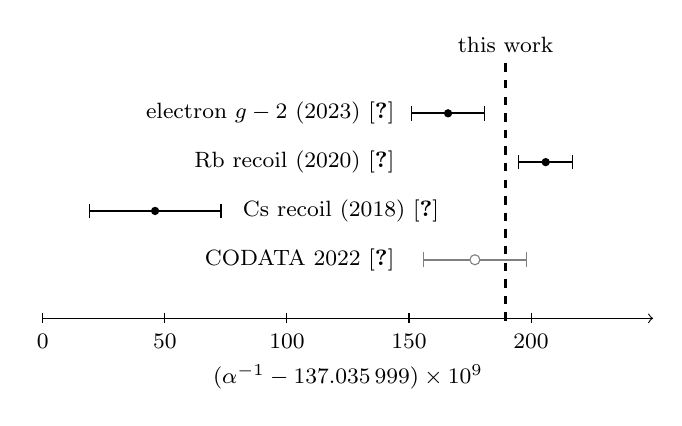
\begin{tikzpicture}[x=0.031cm, y=0.62cm, every node/.style={font=\footnotesize}]
\draw[->] (0,0) -- (250,0);
\foreach \t in {0,50,100,150,200} {\draw (\t,0.1) -- (\t,-0.1); \node[anchor=north] at (\t,-0.12) {$\t$};}
\node[anchor=north] at (125,-0.75) {$(\alpha^{-1} - 137.035\,999)\times 10^{9}$};
\draw[dashed, thick] (189.57,-0.05) -- (189.57,5.25);
\node[anchor=south] at (189.57,5.25) {this work};
\draw[thick] (151,4.2) -- (181,4.2); \draw (151,4.05) -- (151,4.35); \draw (181,4.05) -- (181,4.35); \fill (166,4.2) circle (1.5pt);
\node[anchor=east] at (148,4.2) {electron $g-2$ (2023) \cite{fan2023}};
\draw[thick] (195,3.2) -- (217,3.2); \draw (195,3.05) -- (195,3.35); \draw (217,3.05) -- (217,3.35); \fill (206,3.2) circle (1.5pt);
\node[anchor=east] at (148,3.2) {Rb recoil (2020) \cite{morel2020}};
\draw[thick] (19,2.2) -- (73,2.2); \draw (19,2.05) -- (19,2.35); \draw (73,2.05) -- (73,2.35); \fill (46,2.2) circle (1.5pt);
\node[anchor=west] at (78,2.2) {Cs recoil (2018) \cite{parker2018}};
\draw[thick, gray] (156,1.2) -- (198,1.2); \draw[gray] (156,1.05) -- (156,1.35); \draw[gray] (198,1.05) -- (198,1.35); \draw[gray, fill=white] (177,1.2) circle (1.8pt);
\node[anchor=east] at (148,1.2) {CODATA 2022 \cite{codata2022}};
\end{tikzpicture}
\caption{The inverse of the candidate of Eq.~(\ref{eq:alpha}), $\alpha_{\mathrm{cand}}^{-1} = 137.035\,999\,189\,6\ldots$ (dashed), against the one-standard-deviation intervals of the most precise determinations of $\alpha(0)$: the electron magnetic moment with the Standard Model prediction~\cite{fan2023}, $137.035\,999\,166(15)$; rubidium recoil~\cite{morel2020}, $137.035\,999\,206(11)$; cesium recoil~\cite{parker2018}, $137.035\,999\,046(27)$; and the CODATA 2022 adjustment of such inputs (open circle)~\cite{codata2022}, $137.035\,999\,177(21)$. The exact form carries no uncertainty of its own; it lies $+1.6\sigma$, $-1.5\sigma$, $+5.3\sigma$, and $+0.6\sigma$ from these values.}
\label{fig:comparison}
\end{figure}
